{\color{solution}
\begin{enumerate}
		\item $\textcolor{exampoints}{(1P)}~\text{rank}(A)+\text{dim}(\text{ker}(A))=n~~(\text{for}~A\in\mathbb{R}^{m\times n})$
		\item  \textcolor{exampoints}{(0.5P)}: $A^\top = (U \Sigma V^\top)^\top = V \Sigma^\top U^\top $\\
		\textcolor{exampoints}{(0.5P)}: Since $r = \text{rank}(A) = \text{rank}(A^\top)$ we have
		\begin{align*}
		\text{Im}(A) &= \text{span}\{u_1, \ldots, u_r\}\\
			\text{Im}(A^\top) &= \text{span}\{v_1, \ldots,v_r\}\\
		\end{align*}
			\item 
		$\textcolor{exampoints}{(0.5P)}$ Purpose: Compute eigenvalues of a matrix $A\in\mathbb{R}^{n\times n}$
		\begin{align*}
		\textcolor{exampoints}{(0.5P)}~~A_0&:=A\\
		\text{for}~&i=1,\dots,n\\
		&Q_iR_i:=A_i\\
		&A_{i+1}:=R_iQ_i
		\end{align*}
		\item 
	$\textcolor{exampoints}{(1P)}~$ $R$ is not invertible, because triangular matrices are invertible if and only if all diagonal entries are nonzero (see backward/forward substitution)	
	\item  \textcolor{exampoints}{(1P)}\\
	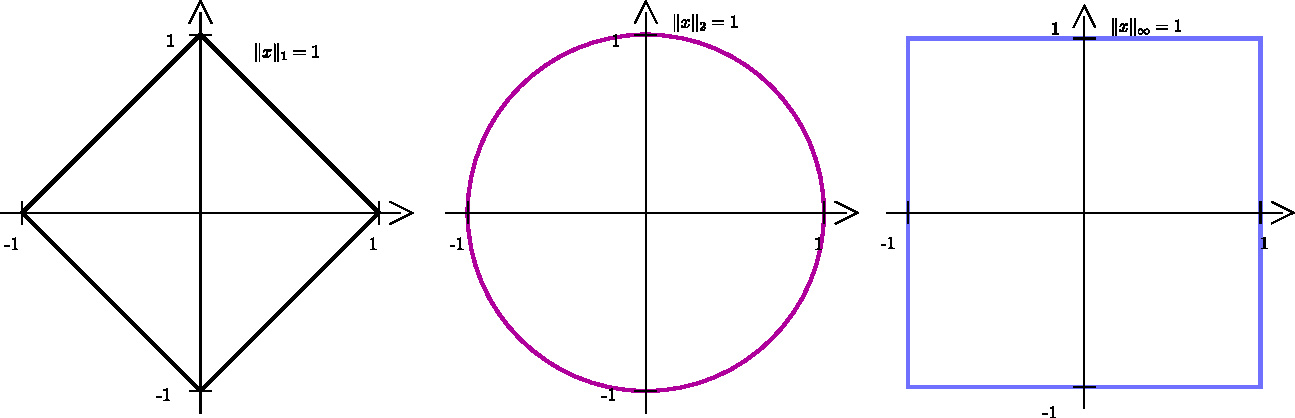
\includegraphics[width=0.35\textwidth]{norms.pdf}
		\item $\textcolor{exampoints}{(0.5P)}~~Q\in\mathbb{R}^{n\times n}$ orthogonal $:\Leftrightarrow~~Q^TQ=I$\\
	$\textcolor{exampoints}{(0.5P)}$ 
	Thus the columns of $Q$ are mutually orthonormal.
\end{enumerate}	
}